%%% Data Analysis and Results
%%%%%%% Wording: ⏳
%%%%%%% Styling: ⏳
%%%%%%% References: ⏳
%%%%% Grammar: ⏳
%%% --------------------------------------------------------------
\chapter{Data Analysis and Results}
\label{ch:data-analysis-and-results}

This chapter presents the data analysis and results of the research.
The goal is to address the research questions outlined earlier, with a focus on providing actionable insights for the event organizer.

The chapter is divided into several sections corresponding to key analytical areas:
\begin{enumerate}
	\item \fullref{sec:analysis-cashflow-and-revenue-sources},
	\item \fullref{sec:analysis-performance-indicators},
	\item \fullref{sec:analysis-beverage-consumption},
	\item and~\fullref{sec:analysis-customers}
\end{enumerate}

Each section focuses on a different aspect of the data analysis trying to answer the research questions, present quantitative results, visualizations, and interpretations.


\section{Cashflow and Revenue Sources Analysis}
\label{sec:analysis-cashflow-and-revenue-sources}

This section provides a comprehensive view of the festival's financial performance and cash flows.
It should answer critical questions about how finances were funded into the system, how were they processed, and what were the final outcomes.

For this analysis, four questions were previously formulated.
However, they were reordered to better fit the narrative of the analysis and logical flow of the chapter:
\begin{enumerate}
	\item \textit{\researchq{cashflow-top-up-balance}}
	\item \textit{\researchq{cashflow-total-sales}}
	\item \textit{\researchq{cashflow-remaining-balance}}
	\item \textit{\researchq{cashflow-total-revenue}}
\end{enumerate}

In the end, this section should provide a clear picture of the financial flows during the event and easy understanding of the generated revenue from various sources.

\subsection{Chip Top-Up Analysis}
\label{subsec:analysis-chip-top-up}
\begin{gray-box}{Research Question}
	\textit{How much and by what means was the balance topped up on the chips?}
\end{gray-box}

Attendees could top up their chip balances via online prepayments or on-site using cash or card.
Additionally, the system allows to top-up~\enquote{artificial} credit for VIP-issued chips which is also a mean of funding the system.
However, these VIP credits are later not refundable, but this will be discussed in the next section.

This subsection quantifies these methods, highlighting their respective contributions to the overall top-up total.

To get the results, it was necessary to find all top-up transactions and their respective payment methods used.
This resulted in \bfmtnum{17704}~top-up transactions, with a total value of~\bfmtczk{14520973}.

When looking at the grouping by payment methods, the results in~\autoref{fig:top-up-transactions-by-payment-method} give a clear picture of the distribution.

\begin{figure}[H]
	\centering
	% First the pie chart
	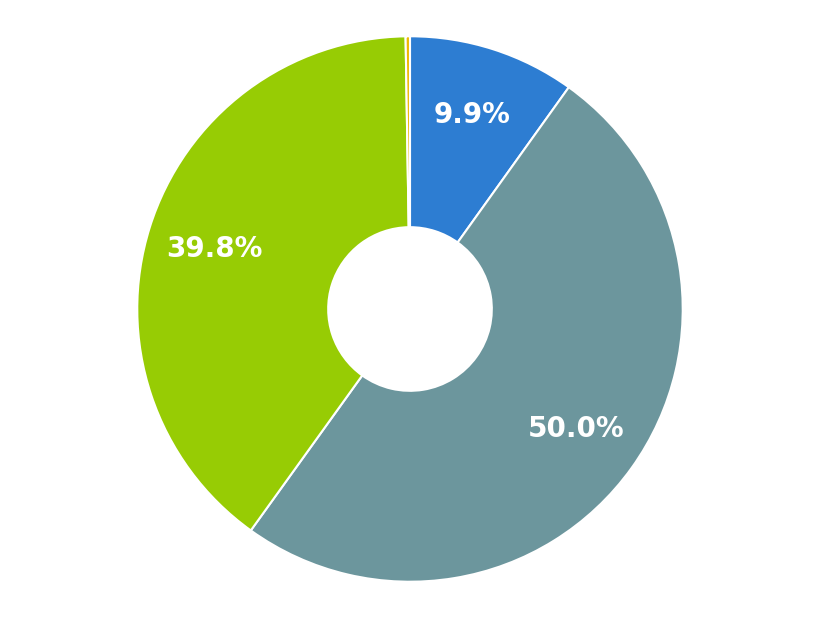
\includegraphics[width=0.75\textwidth]{\ThesisFigures/charts/topup-methods}
	\vspace{1em}  % add some space between chart and table

	% Then the table
	\small
	\begin{tabular}{@{}lrr@{}}
		\toprule
		\textbf{Payment Method}                & \textbf{Count} & \textbf{Total Value (CZK)} \\
		\midrule
		\colorindicator{chart2}Card terminal     & \fmtnum{8486}  & \fmtczk{7264503}           \\
		\colorindicator{chart3}Cash              & \fmtnum{7561}  & \fmtczk{5782570}           \\
		\colorindicator{chart1}Online pre top-up & \fmtnum{1634}  & \fmtczk{1436400}           \\
		\colorindicator{chart4}VIP issued        & \fmtnum{23}    & \fmtczk{37500}             \\
		\bottomrule
	\end{tabular}
	\caption{Top-Up Transactions by Payment Method}
	\label{fig:top-up-transactions-by-payment-method}
\end{figure}

Thanks to the results, it is clear how many funds did the system receive and by what means.

\begin{blue-box}{Key Takeaways}
	\begin{itemize}
		\item Total top-up amount was~\bfmtczk{14520973}.
		\item Most used payment method was card terminal at the event with 50\% of all top-ups.
		\item Only around 10\% of the top-ups were done online.
	\end{itemize}
\end{blue-box}

\subsection{Sales Analysis}
\label{subsec:analysis-sales}
\begin{gray-box}{Research Question}
	\textit{What was the total sales of the event, how much of it was the sales of the organizer and how many external vendors?}
\end{gray-box}

The sales analysis was crucial for understanding the overall sales behavior and served as a basis for further insights tightly connected to the revenue sources.

To answer the research question, it was necessary to find all sales transactions and their respective sellers and to divide them into two groups: the direct organizer's sales and external vendors' sales.
And for better understanding, the sales were also grouped by the product categories (see~\autoref{tab:product-categories} for the list of categories).

The results show that the total sales of the event were~\bfmtczk{11711807} with the organizer's sales being~\bfmtczk{8240264} and the external vendors' sales~\bfmtczk{3471543}.

The organizer, most importantly, sold all the beer beverages and most of the non-alcoholic and alcoholic (spirits) beverages.
Whereas the external vendors sold mainly the food, wine beverages and other uncategorized products.
This can be seen in~\autoref{fig:sales-organizer-vs-vendors} below.

\begin{figure}[H]
	\centering
	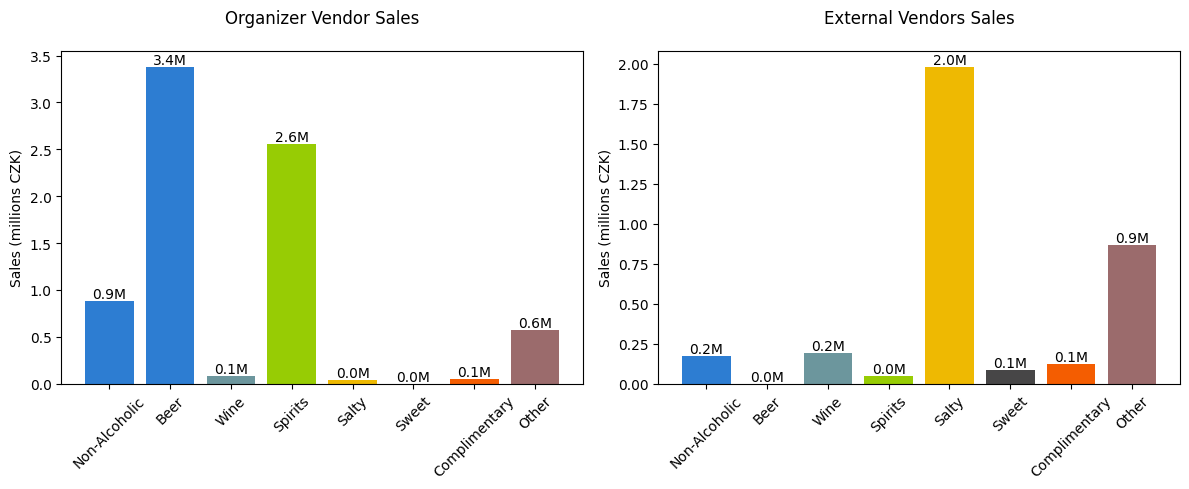
\includegraphics[width=0.99\textwidth]{\ThesisFigures/charts/sales-vendors}
	\caption{Sales of the Organizer vs. External Vendors}
	\label{fig:sales-organizer-vs-vendors}
\end{figure}

The organizer also sold not so little of uncategorized products, which after further investigation turned out to be ticket sales at the event amounting to~\bfmtczk{684700}.

In total, the organizer direct sales were \textbf{70\%} of the total sales, which is a significant portion, and thus the organizer itself has even bigger influence on the event's financial performance.

\begin{blue-box}{Key Takeaways}
	\begin{itemize}
		\item Total sales of the event were~\bfmtczk{11711807}, where organizer sales were~\textbf{70\%} of the total.
		\item The organizer sold all beer beverages and the majority of the non-alcoholic and alcoholic beverages.
		\item The organizer also sold tickets at the event amounting to~\bfmtczk{684700}.
		\item External vendors sold mainly food, wine beverages, and other uncategorized products.
	\end{itemize}
\end{blue-box}

\subsection{Remaining Chip Balances}
\label{subsec:analysis-remaining-balances}
\begin{gray-box}{Research Question}
	\textit{How much balance remained on all chips after the event and after refunds?}
\end{gray-box}

The remaining chip balances are crucial for the event organizer as they represent the potential revenue that can be still claimed.
Any unclaimed balances after a given refund period, which is usually up to 14~days after the event will be considered as organizer's taxable revenue.

Out of the total top-up amount of~\bfmtczk{14520973}, the total spent credit amounted to~\bfmtczk{10984945}, which left a total of~\bfmtczk{3536028} on the chips before refunds.
After refunds – done both at the event (\bfmtczk{15379}) and later via online bank refund requests (\bfmtczk{3163567}) – the remaining balance was reduced to~\bfmtczk{357082}.

However, this still included the artificially issued VIP credits with leftover balance of~\bfmtczk{12405}.
The system also reported integrity errors in the data, which resulted in a total of~\bfmtczk{10246} due to fraudulent activities performed by some attendees which were automatically suspended by the system.

This left the total unclaimed balance at~\bfmtczk{334431}, which has been claimed by the organizer as taxable revenue.

Since these numbers can be quite abstract, the results in a form of sankey diagram in~\autoref{fig:remaining-balances-sankey} below provide a clear picture of the flow of the funds.

\begin{figure}[H]
	\centering
	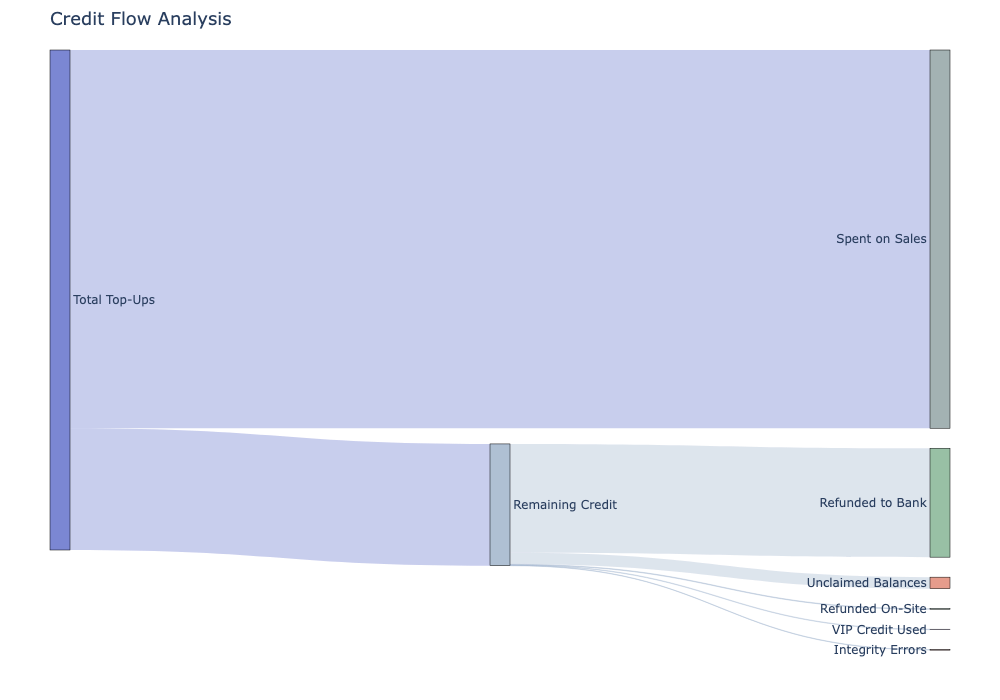
\includegraphics[width=0.99\textwidth]{\ThesisFigures/charts/balances-sankey}
	\caption{Remaining Chip Balances Sankey Diagram}
	\label{fig:remaining-balances-sankey}
\end{figure}

Thanks to this breakdown, it is clear how the remaining balances were reduced and what was the final outcome.
These results are important for the last part of this section, which is the total revenue of the organizer.

\begin{blue-box}{Key Takeaways}
	\begin{itemize}
		\item Total unused credit was~\bfmtczk{3536028}.
		\item Credit refunded to customers was~\bfmtczk{3178946}.
		\item After VIP issued credits and system integrity error, the unclaimed balance was~\bfmtczk{334431}.
	\end{itemize}
\end{blue-box}

\subsection{Total Revenue of the Organizer}
\label{subsec:analysis-total-revenue}
\begin{gray-box}{Research Question}
	\textit{What was the total revenue of the organizer and what does it consist of?}
\end{gray-box}

The festival's financial model is based on a combination of revenue streams.

The most important stream is the \textbf{commission from the vendor sales}, which is arranged in advance between the organizer and the vendors.
The commission is, in this case, a percentage (ranging from 15\% to 30\% depending on the deal) of the vendor sales amount without VAT\@.

Therefore, this required finding all sales transactions made at the external vendors' stands and calculating the commission based on the agreed percentage.
However, this was not a straightforward task, since a transaction could contain multiple products even from different vendors.

This required a more complex calculation, for which was used the previously mentioned data processing views which were designed for this purpose.
In the end, the total revenue from sales commissions was~\bfmtczkp[2]{820712,79}.

Another source of revenue is the \textbf{unclaimed chip balances}, which, after a credit refund period, are considered as taxable revenue for the organizer.
This, thanks to the previous subsection, was found to be~\bfmtczk{334431}.

\begin{figure}[H]
	\centering
	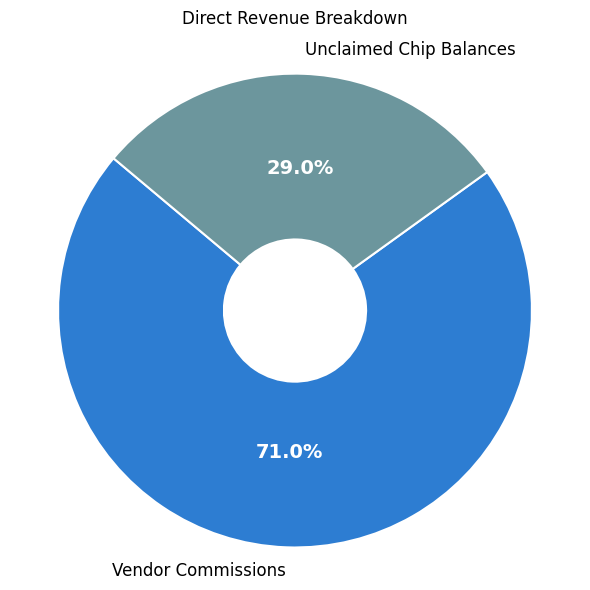
\includegraphics[width=0.48\textwidth]{\ThesisFigures/charts/revenue-sources-direct}
	\caption{Breakdown of Direct Revenue Streams}
	\label{fig:revenue-breakdown-direct}
\end{figure}

Currently totalling~\bfmtczkp[2]{1155143,79} is the direct revenue of the organizer from the event and can be seen in~\autoref{fig:revenue-breakdown-direct} above.

However, given the circumstances and setup of this event, there were also additional, but indirect revenue streams that were not included in the total revenue.
These include \textbf{the online ticket sales}, which were sold by the organizer and \textbf{the direct sales of the organizer}.
They were not included in the total direct revenue, as they may misinterpret the results since the analysis lacks expenses of the organizer.

If we were to include these, the total revenue would increase by~\bfmtczk{11179700} from the online ticket sales and~\bfmtczk{8240264} from the direct sales, which would result in a total revenue of~\bfmtczkp[2]{20575107,79}.

To better understand the revenue streams, the results are visualized in~\autoref{tab:revenue-summary-breakdown} and in~\autoref{fig:revenue-breakdown-total} below.

\begin{table}[H]
	\centering
	\begin{tabularx}{\textwidth}{|>{\columncolor{unicorn_blue!5}}X|>{\columncolor{unicorn_blue!5}}r|}
		\hline
		\rowcolor{unicorn_blue}
		\textbf{\color{white}Revenue Stream}         & \textbf{\color{white}Amount (CZK)} \\
		\hline
		\hline
		\colorindicator{chart1}Vendor Commissions      & \fmtczkp[2]{820712.79}             \\
		\colorindicator{chart2}Unclaimed Chip Balances & \fmtczk{334431}                    \\
		\hline
		\textbf{Total Direct Revenue}                  & \bfmtczkp[2]{1155143.79}           \\
		\hline
		\colorindicator{chart3}Online Ticket Sales     & \fmtczk{11179700}                  \\
		\colorindicator{chart4}Organizer Direct Sales  & \fmtczk{8240264}                   \\
		\hline
		\textbf{Total Revenue (All Streams)}           & \bfmtczkp[2]{20575107.79}          \\
		\hline
	\end{tabularx}
	\caption{Revenue Summary Breakdown}
	\label{tab:revenue-summary-breakdown}
\end{table}

\begin{figure}[H]
	\centering
	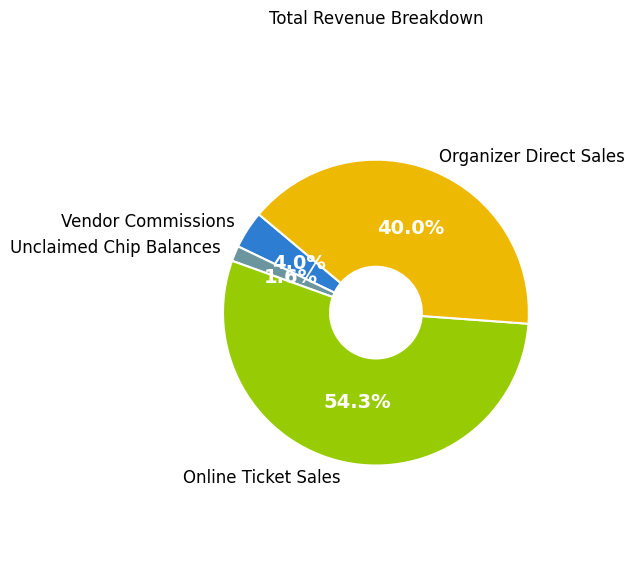
\includegraphics[width=0.75\textwidth]{\ThesisFigures/charts/revenue-sources-total}
	\caption{Breakdown of All Revenue Streams}
	\label{fig:revenue-breakdown-total}
\end{figure}

\begin{blue-box}{Key Takeaways}
	\begin{itemize}
		\item Total direct revenue of the organizer was~\bfmtczkp[2]{1155143,79}.
		\item Vendor sale commission contributed to~approximately 71\% of the total direct revenue.
		\item With other indirect revenue streams, the total revenue would be~\bfmtczkp[2]{20575107,79}.
	\end{itemize}
\end{blue-box}

\subsection{Summary}
\label{subsec:analysis-cashflow-summary}

This section provided a comprehensive view of the festival's financial performance and cash flows.
The results covered the top-up transactions, sales analysis, remaining chip balances, and the total revenue of the organizer and contributed to a better understanding from the financial perspective of the festival.

Nevertheless, results covered in these subsections are only a part of the whole picture and can be interpreted in various ways.

For this particular challenge, a summarized cash flow diagram of payments was created, containing thus only the direct revenue streams.
This diagram can be seen in the~\autoref{fig:cash-flow-diagram} below.

\begin{figure}[H]
	\centering
	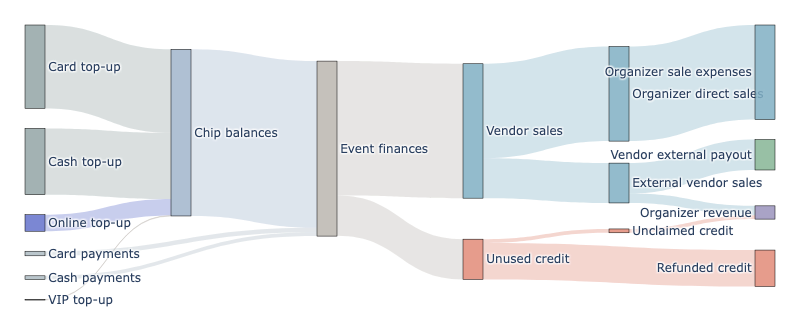
\includegraphics[width=0.99\textwidth]{\ThesisFigures/charts/revenue-cash-flows}
	\caption{Overall Cash Flow Diagram}
	\label{fig:cash-flow-diagram}
\end{figure}

This diagram provides a clear overview of the financial flows during the festival and nicely summarizes the results of this analysis.


\section{Performance Indicators Analysis}
\label{sec:analysis-performance-indicators}
\todo{Haha.}


\section{Beverage Consumption Analysis}
\label{sec:analysis-beverage-consumption}
\todo{Haha.}


\section{Customer Analysis}
\label{sec:analysis-customers}
\todo{Haha.}

